\exer{[EQD-002]}
\setcounter{numques}{0}~\\

\section{Etude d'un trafic routier}

Ce sujet concerne la conception d'un logiciel d'étude de trafic routier. On modélise le déplacement d'un ensemble de voitures sur des files à sens unique (voir Figures~\ref{f_exemple_une_file} et~\ref{f_exemple_deux_file}). C'est un
schéma simple qui peut permettre de comprendre l'apparition d'embouteillages et de concevoir des
solutions pour fluidifier le trafic.

\begin{figure}[!htb]
\begin{minipage}{0.45\textwidth}
\begin{center}

\includegraphics[width=1.0\textwidth]{fig1.jpg}
\caption{\label{f_exemple_une_file} Représentation d'une file de
longueur onze comprenant quatre voitures, situées
respectivement sur les cases d'indices 0, 2, 3 et 10.}
\end{center}
\end{minipage}
\begin{minipage}{0.45\textwidth}
\begin{center}
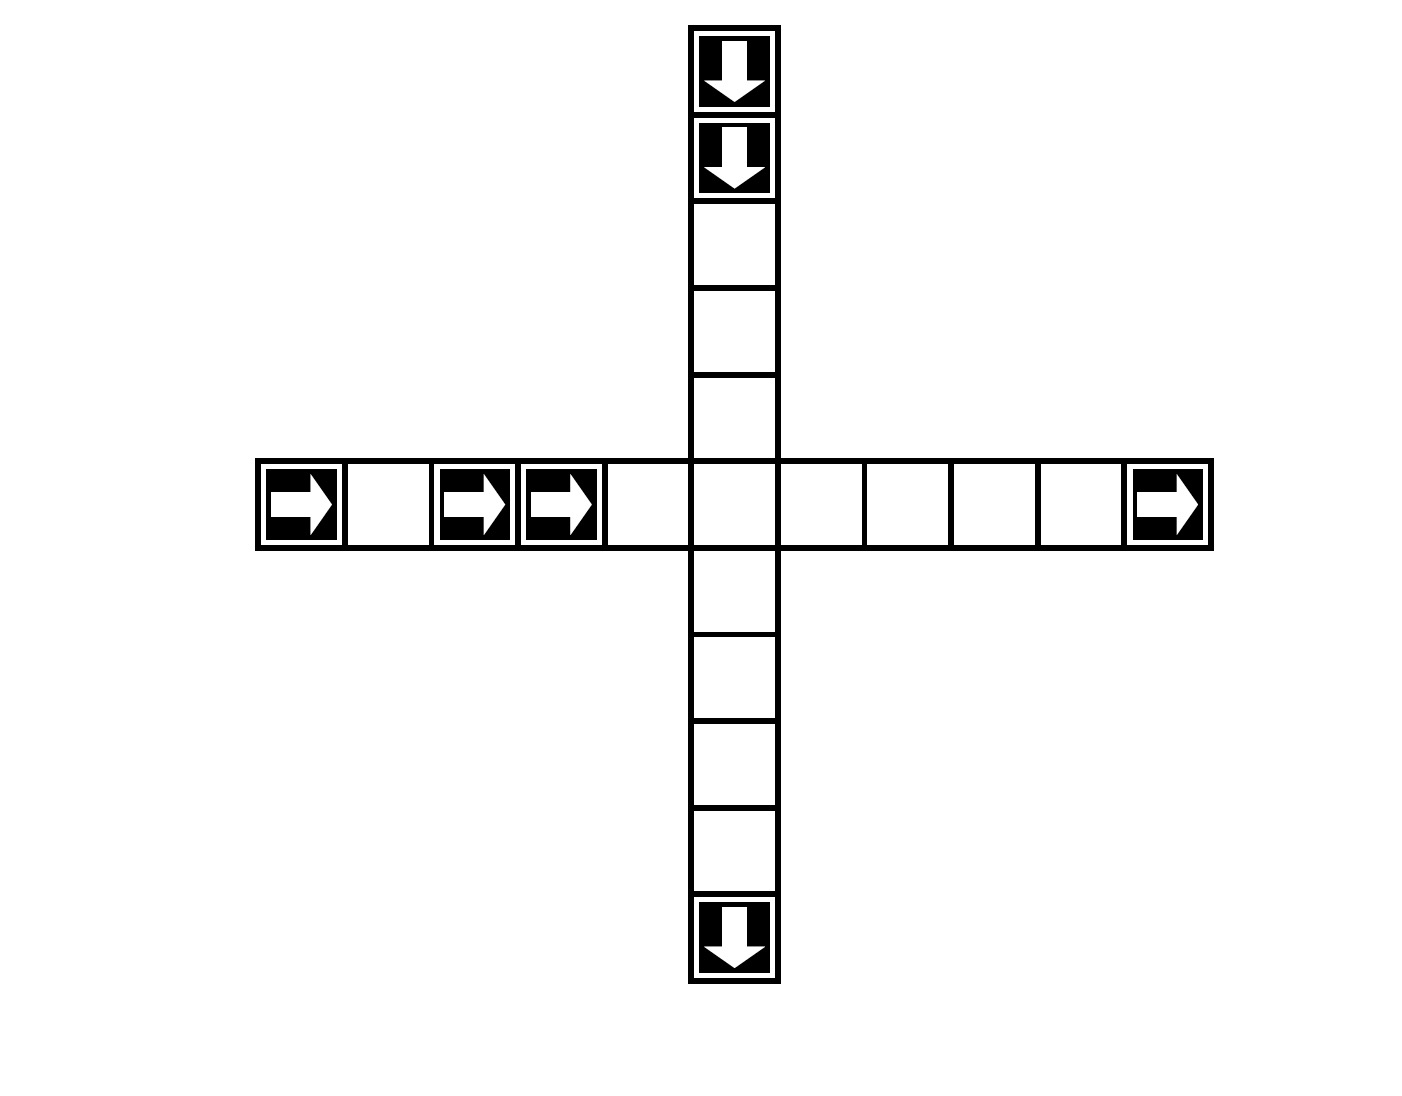
\includegraphics[width=1.0\textwidth]{fig2.jpg}
\caption{\label{f_exemple_deux_file} Configuration représentant deux files de circulation à sens unique se croisant en une case. Les voitures sont représentées par un carré noir.}
\end{center}
\end{minipage}
\end{figure}

\subsection{Préliminaires}



Dans un premier temps, on considère le cas d'une seule file, illustré par la Figure~\ref{f_exemple_une_file}. Une file de
longueur $n$ est représentée par $n$ cases. Une case peut contenir au plus une voiture. Les voitures
présentes dans une file circulent toutes dans la même direction (sens des indices croissants, désigné
par les flèches sur la Figure~\ref{f_exemple_une_file}) et sont indifférenciées.


\question{} Expliquer comment représenter une file de voitures à l'aide d'une liste de booléens.

\question{} Donner une ou plusieurs instructions \lstinline{Python} permettant de définir une liste $A$ représentant la file de voitures illustrée par la Figure~\ref{f_exemple_une_file}.

\question{} Soit $L$ une liste représentant une file de longueur $n$ et $i$ un entier tel que $0\leqslant i < n$.
Définir en Python la fonction \lstinline{occupe(L, i)} qui renvoie \lstinline{True} lorsque la case d'indice $i$ de la file
est occupée par une voiture et \lstinline{False} sinon.

\question{} Combien existe-t-il de files différentes de longueur $n$ ? Justifier votre réponse.

\question{} \'Ecrire une fonction \lstinline{egal(L1, L2)} retournant un booléen permettant de savoir si deux listes $L1$ et $L2$ sont égales.

\question{} Que peut-on nom\_de\_fichier de la complexité de cette fonction ?


\subsection{ Base de données}

On modélise ici un réseau routier par un ensemble de croisements et de voies reliant ces croisements.
Les voies partent d'un croisement et arrivent à un autre croisement. Ainsi, pour modéliser une route
à double sens, on utilise deux voies circulant en sens opposés.
La base de données du réseau routier est constituée des relations suivantes :
\begin{itemize}
	\item[\textbullet]  Croisement(\underline{id}, longitude, latitude)
    \item[\textbullet] Voie(\underline{id}, longueur, id\_croisement\_debut, id\_croisement\_fin)
\end{itemize}

Dans la suite on considère $c$ l'identifiant (id) d'un croisement donné.

\question{} \' Ecrire la requête SQL qui renvoie les identifiants des croisements atteignables en utilisant une seule voie à partir du croisement ayant l'identifiant c.

\question{} \'Ecrire la requête SQL qui renvoie les longitudes et latitudes des croisements atteignables en utilisant une seule voie, à partir du croisement c.

\question{} Que renvoie la requête SQL suivante?

% \lstinputlisting{req_sql.sql}

\subsection{Simulation dynamique}
 
On introduit les bibliothèques \texttt{Math} et \texttt{NumPy} à l'aide des lignes suivantes~:
\begin{lstlisting}
import math as m
import numpy as np
\end{lstlisting}

%%%%%%%%%%%%
% Intérêt de math ? %
%%%%%%%%%%%%

On s'intéresse maintenant à l'apparition des voitures en début de file. On se place alors dans le cas d'un parking lors d'une sortie d'usine entre 17 h et 19 h. Afin de simplifier le problème on considère qu'à $t=0$, il est 17 h et à $t=1$, il est 19 h.

Tous les employés de l'usine ne sortent pas au même moment.  On donne sur la Figure~\ref{f_quitte_stat} l'évolution de $Q(t)$ qui représente le nombre de véhicules quittant le stationnement par unité de temps, pour $t\in[0,1]$. On considère que cette fonction est nulle en dehors de cet intervalle. On appelle \texttt{db\_stat\_max} le maximum de $Q$ entre 0 et 1.

\[ \forall t\in[0,1],\ Q(t)=\mbox{\texttt{db\_stat\_max}}\cdot \mathrm e^{\left(\displaystyle 1-\frac{1}{4t(1-t)}\right)}\]

\begin{figure}[!htb]
\begin{center}
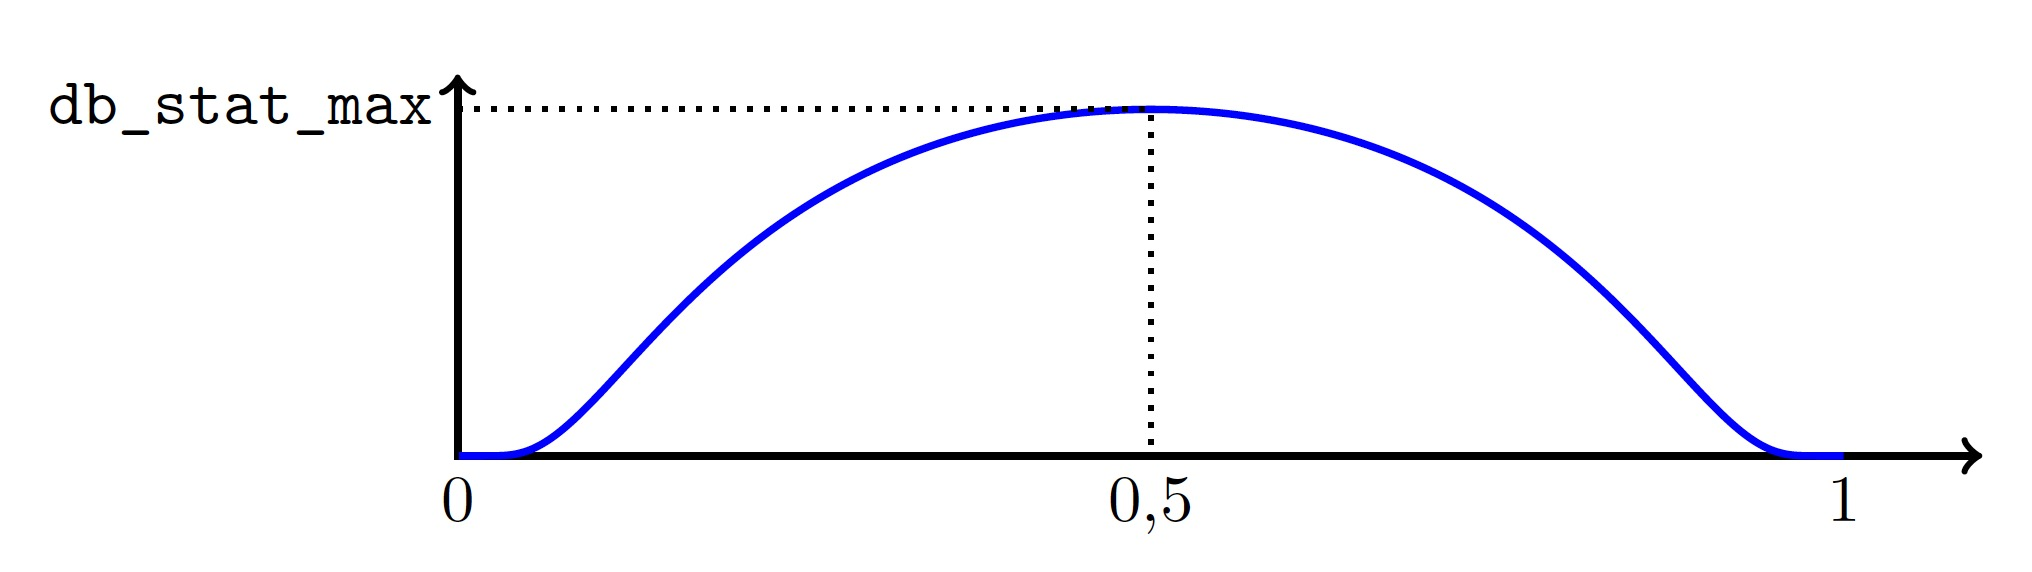
\includegraphics[width=0.8\textwidth]{fig3.jpg}
\caption{\label{f_quitte_stat} Évolution du nombre de véhicules quittant le stationnement par unité de temps}
\end{center}
\end{figure}


\question{} \'Ecrire une fonction \texttt{Q(t)} permettant d'obtenir, pour tout réel $t$, le nombre de véhicules quittant le stationnement par unité de temps. On considère \texttt{db\_stat\_max} comme une variable globale. Faire attention aux cas où \texttt{t = 0} et \texttt{t = 1}. 

\question{} \' Ecrire une fonction \texttt{integrale(f, a, b, n)} permettant,  avec la méthode des trapèzes, d'estimer l'intégrale de \texttt{f} entre \texttt{a} et \texttt{b} à partir de \texttt{n} points équirépartis.

\question{} On appelle $N(t)$ le nombre de véhicules ayant quitté le stationnement jusqu'à l'instant $t$. \'Ecrire une fonction \texttt{Nb(t, n)} renvoyant une valeur approchée de ce nombre, en utilisant $n$ points. 
	
\emph{La suite de cette partie permettant d'obtenir $N(t)$ par une autre méthode, la fonction \texttt{Nb} ne sera plus utilisée.}

La vitesse de sortie des véhicules est limitée par le nombre de véhicules sortants. En effet, quand peu de véhicules sortent du parking, ces derniers peuvent circuler à vitesse maximale $V_{max}$. En revanche, lorsque beaucoup de véhicules sont en mouvement, ces derniers se ralentissent les uns les autres. On appelle $K$ la concentration de véhicules cherchant à rejoindre la sortie du parking à un instant donné et $K_{sat}$ le nombre de véhicules à partir duquel la vitesse de sortie est minimale ($V_{min}$).

L'expression de la vitesse des véhicules $V$ en fonction de $K\in[0,K_{sat}]$ est donnée par
\[V(K)=\frac{V_{max}-V_{min}}{2}\cdot\left(1+\cos\left(\pi\cdot\frac{K}{K_{sat}}\right)\right)+V_{min}.\]

\question{} \'Ecrire une fonction \texttt{V(K)} prenant en entrée un flottant \texttt{K} et renvoyant la valeur de la vitesse correspondante. On considère \texttt{Vmin}, \texttt{Vmax} et \texttt{Ksat} comme des variables globales. 


La conservation du nombre total de véhicules conduit au système différentiel suivant :
\begin{align}
\frac{\mathrm{d} N}{\mathrm{d} t}(t)&=Q(t) \label{eq:NbPlusStat}\\
\frac{\mathrm{d} K}{\mathrm{d} t}(t)&= Q(t)-K(t)\cdot V(K)\\\smallskip
\frac{\mathrm{d} S}{\mathrm{d} t}(t)&= K(t)\cdot V(K)\label{eq:Sortis}
\end{align}
où $S(t)$ désigne le nombre de véhicules sortis du parking à l'instant $t$.

\question{} Rappeler la relation de récurrence de la méthode d'Euler explicite pour un problème défini par son équation différentielle $y'(t)=F(y(t), t)$ avec $h=\Delta t$ le pas de temps supposé constant.

On considère que cette méthode est implémentée dans une fonction \texttt{odeint(F, Y0, T)} où \texttt{F} est la fonction associée au problème de Cauchy, \texttt{Y0} est un tableau \texttt{NumPy} contenant les valeurs initiales de la fonction $Y$ et \texttt{T} un tableau \texttt{NumPy} contenant les différents pas de temps.
\medskip

\noindent
\begin{figure}[!htb]
\begin{minipage}{0.48\textwidth}

On cherche à vectorialiser les équations (\ref{eq:NbPlusStat}) à (\ref{eq:Sortis}) et on pose \[Y(t)=\begin{pmatrix}N(t)\\ K(t)\\ S(t)\end{pmatrix}.\]
On rappelle qu'une liste \texttt{L} peut être convertie en tableau \texttt{NumPy} en utilisant
\texttt{T = np.array(L)}.

\question{} \' Ecrire une fonction \texttt{F\_Parking(Y, t)} permettant de simuler les équations  (\ref{eq:NbPlusStat}) à (\ref{eq:Sortis}) à partir de la fonction \texttt{odeint}.

La Figure~\ref{f_parking} donne une simulation de la sortie des véhicules du parking d'une usine avec\linebreak
 \texttt{dbstatmax = 200}, \texttt{Vmin = 4}, \texttt{Vmax = 24} et \texttt{Ksat = 18}.
\end{minipage}\hfill
\begin{minipage}{0.48\textwidth}
\begin{center}
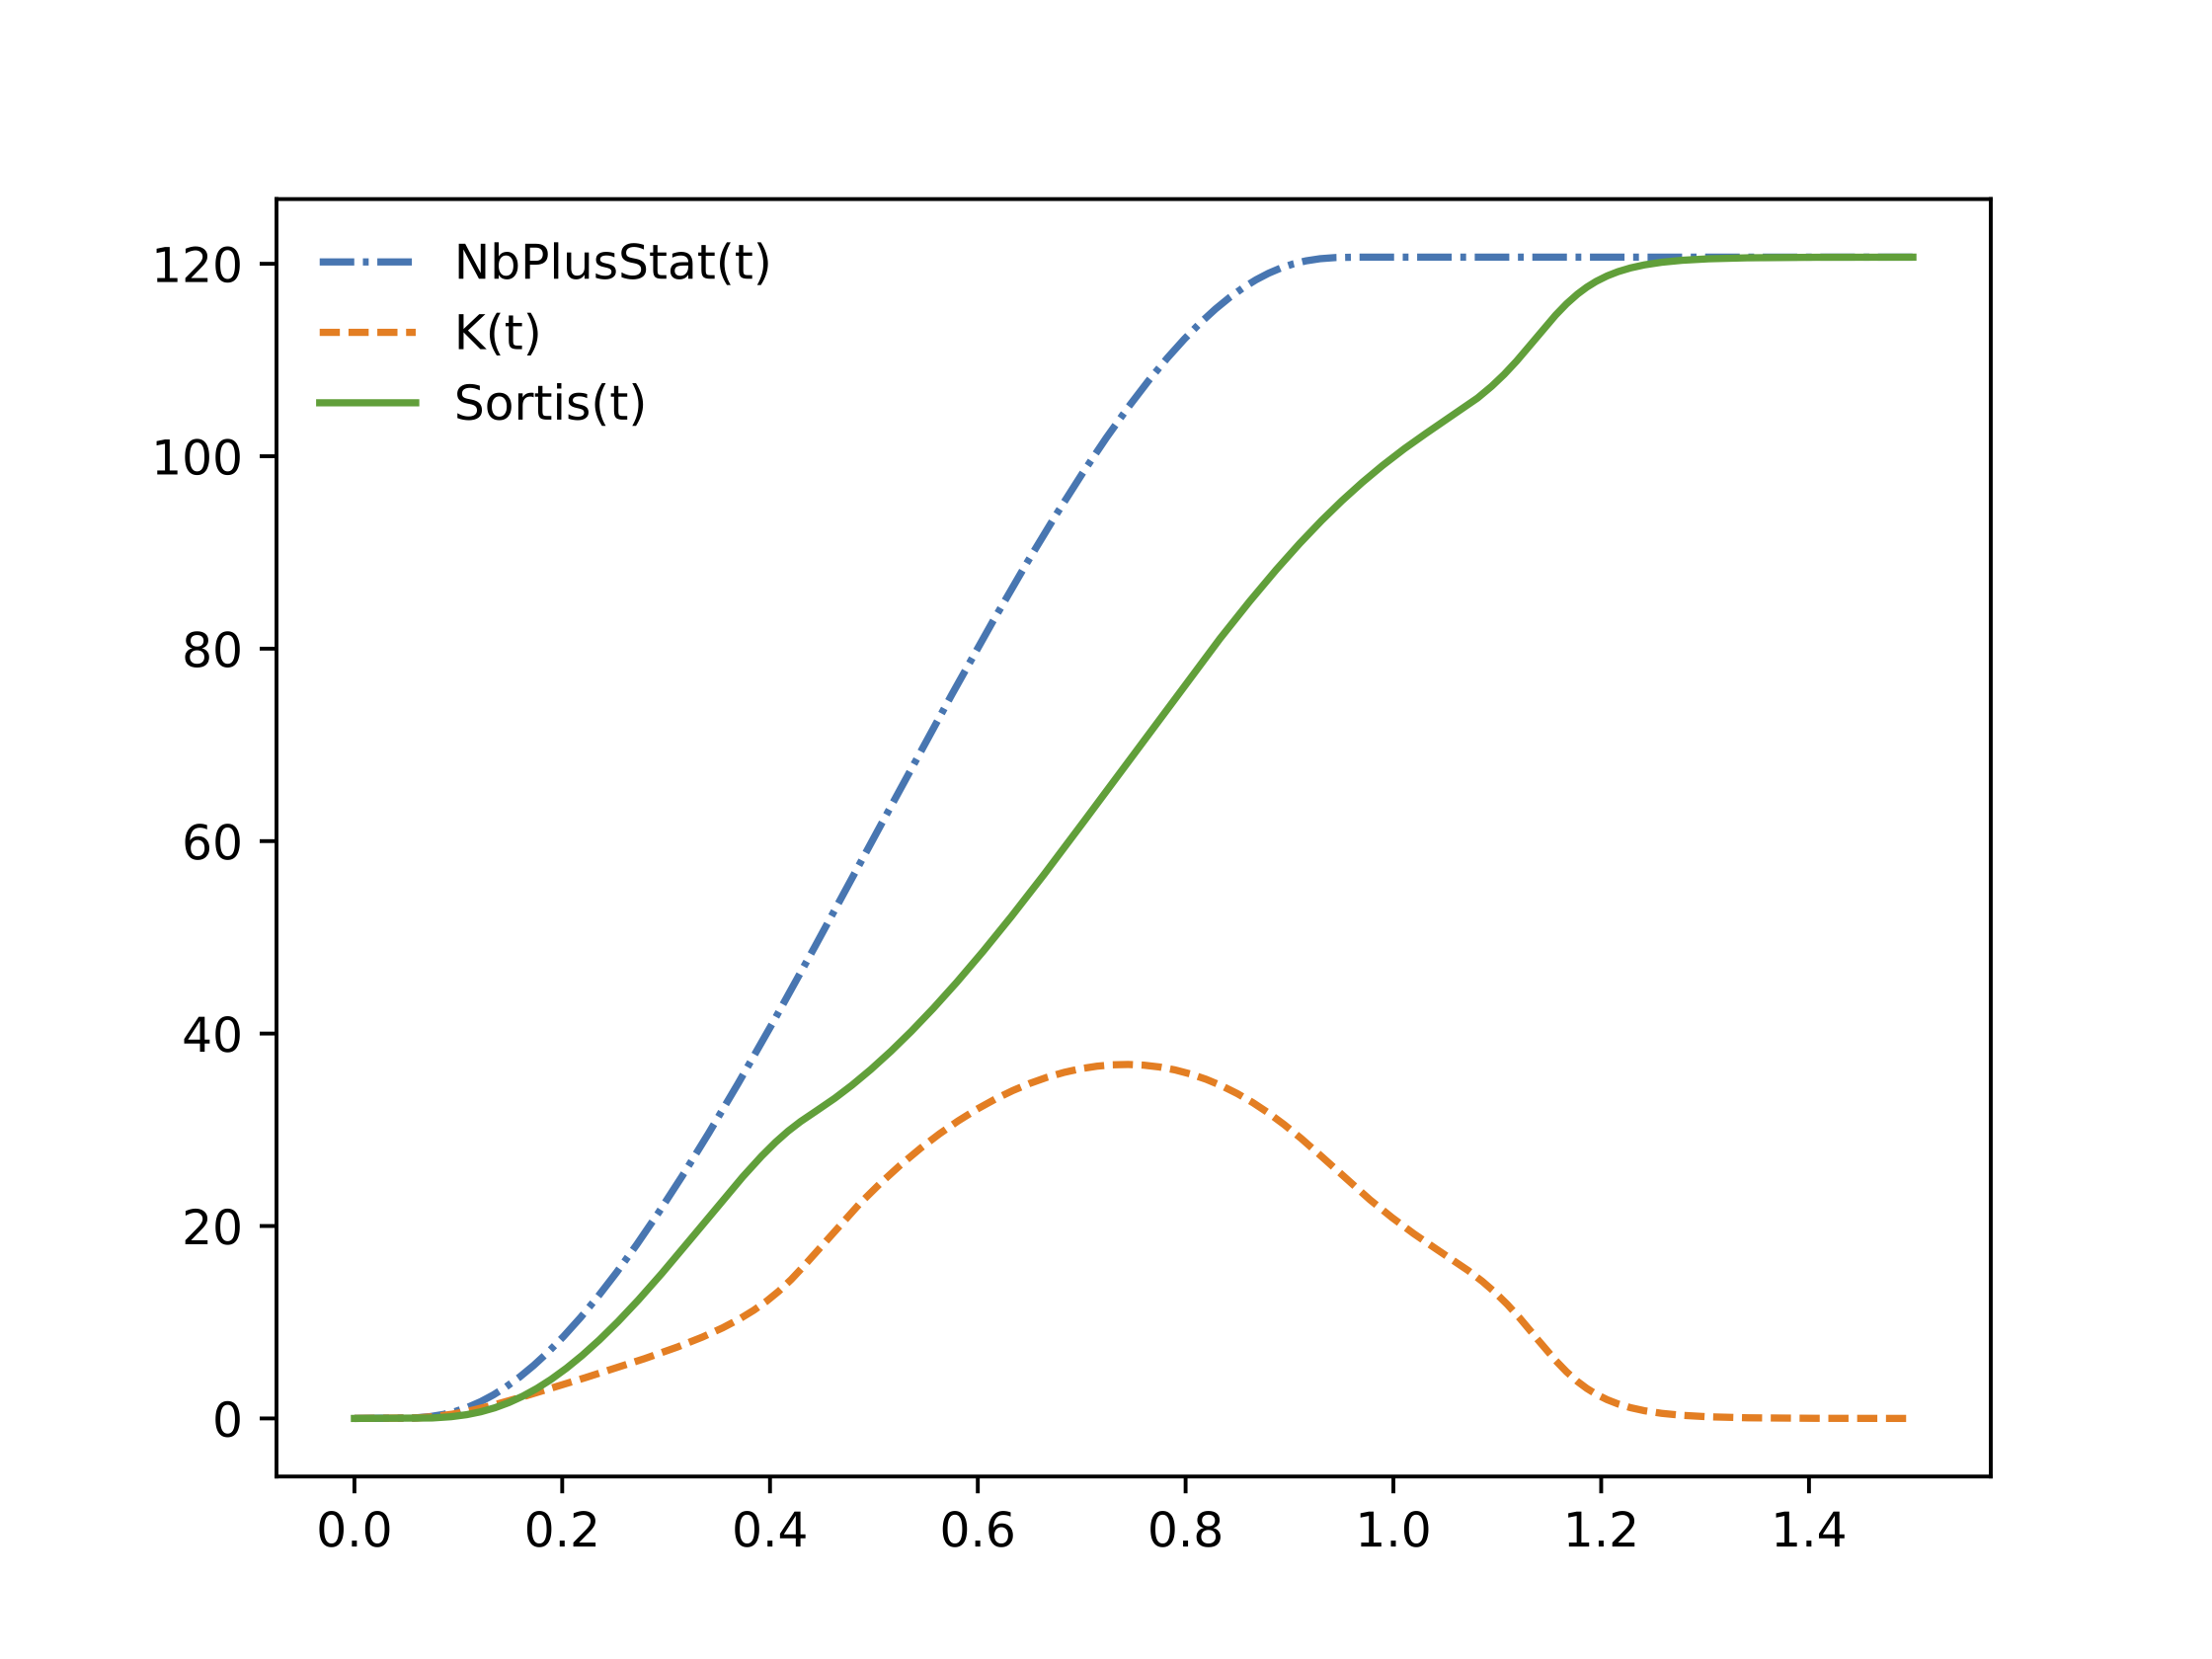
\includegraphics[width=1.0\textwidth]{Simulations-parking}
\caption{\label{f_parking} Simulation de la sortie des véhicules du parking d'une usine}
\end{center}
\end{minipage}
\end{figure}


\question{} Commenter en quelques lignes les allures des courbes de la Figure~\ref{f_parking}.
